\SourcePage{GELFAND-P000450}{unlabelled}
\uuline{\mbox{$25/\underline{\overline{\mathrm{IX}}}$}-72\,yr.}
\quad\uuline{Gabrielov.}

Fam. of Hodge structures over $S$ (nonsingular analyt. set)
\Unclear{GELFAND-P000450}{non-singular-word}{Two rounded strokes are joined after “б”. The reading is “неособое” (“nonsingular”).}
\end{GelfandAdjacentEvidence}
\begin{GelfandAdjacentEvidence}{GELFAND-P000450}{2}


$1)$ $\mathcal H_{\mathbb Z}$ — loc. free sheaf of $\mathbb Z$-modules of fin. type.

\sout{2)}\quad From it constr. a loc. triv. compl. bundle $H_{\mathbb C}$.
\Unclear{GELFAND-P000450}{cancelled-number}{The cancelled beginning of the line is provisionally read as “2)”.}
\end{GelfandAdjacentEvidence}
\begin{GelfandAdjacentEvidence}{GELFAND-P000450}{3}


\SourceFigure{GELFAND-P000450}{deligne-annotation}{An arrow from the complex scalar extension points to the note. The lower line of the note turns up at its left end.
\par\smallskip\centering\color{black}
\begingroup\color{black}\GelfandFitDiagram{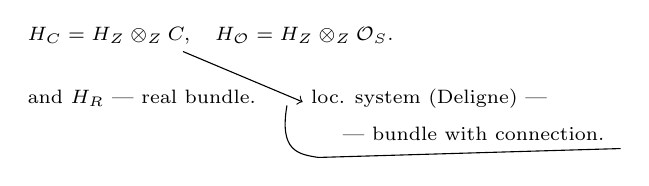
\begin{tikzpicture}[x=1mm,y=1mm,every node/.style={font=\scriptsize,inner sep=0pt,anchor=base west}]
\node (complex) at (0,16)
  {$H_{\mathbb C}=H_{\mathbb Z}\otimes_{\mathbb Z}\mathbb C,$};
\node at ([xshift=3mm]complex.base east)
  {$H_{\mathcal O}=H_{\mathbb Z}\otimes_{\mathbb Z}\mathcal O_S$.};
\node at (0,8) {and $H_{\mathbb R}$ — real bundle.};
\node (localsystem) at (36,8) {loc. system (Deligne) —};
\node (bundle) at (40,3.4) {— bundle with connection.};
\draw[->] ([xshift=-1mm,yshift=-.8mm]complex.south east)
  -- ([xshift=-1mm,yshift=.25mm]localsystem.base west);
\draw (33,7.8) .. controls (32,2) and (34.4,1.6) .. (37,1.2)
  -- ([xshift=2mm,yshift=-1mm]bundle.south east);
\end{tikzpicture}}\endgroup}
\end{GelfandAdjacentEvidence}
\begin{GelfandAdjacentEvidence}{GELFAND-P000450}{4}


$2)$ in $H_{\mathbb C}$ a decreasing filtration by holom. bundles
\[
H_{\mathbb C}=F^0\supset F^1\supset\ldots\supset F^n
\]

\SourceFigure{GELFAND-P000450}{connection-bubble}{A loop encloses the inserted “есть” (“there is”).
\par\smallskip\centering\color{black}
\begingroup\color{black}\GelfandFitDiagram{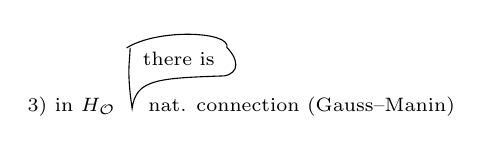
\begin{tikzpicture}[x=1mm,y=1mm,every node/.style={font=\scriptsize,inner sep=0pt,anchor=base west}]
\node (prefix) at (0,4) {$3)$ in $H_{\mathcal O}$};
\node (natural) at ([xshift=4mm]prefix.base east) {nat. connection (Gauss–Manin)};
\node (exists) at ([xshift=-.7mm,yshift=5.8mm]natural.base west) {there is};
\coordinate (tail) at ([xshift=-2mm,yshift=.4mm]natural.base west);
\draw ([xshift=-2mm,yshift=.5mm]exists.north west)
  .. controls ([xshift=2mm,yshift=3mm]exists.north west) and
              ([xshift=2mm,yshift=2.6mm]exists.north east) ..
              ([xshift=1.5mm,yshift=.55mm]exists.north east)
  .. controls ([xshift=3mm,yshift=-1mm]exists.north east) and
              ([xshift=3.1mm,yshift=-.8mm]exists.south east) ..
              ([xshift=1.2mm,yshift=-1.2mm]exists.south east)
  .. controls ([xshift=2mm,yshift=-1.5mm]exists.south west) and
              ([xshift=-.8mm,yshift=-1.6mm]exists.south west) .. (tail)
  .. controls ([xshift=-2mm,yshift=-.6mm]exists.south west) and
              ([xshift=-1.6mm,yshift=.5mm]exists.south west) ..
              ([xshift=-1.55mm,yshift=.5mm]exists.north west);
\end{tikzpicture}}\endgroup}
\end{GelfandAdjacentEvidence}
\begin{GelfandAdjacentEvidence}{GELFAND-P000450}{5}

\Unclear{GELFAND-P000450}{connection-name}{The middle letters of the first name are joined. The pair is read as “Гаусса—Манина” (“Gauss–Manin”).}
\end{GelfandAdjacentEvidence}
\begin{GelfandAdjacentEvidence}{GELFAND-P000450}{6}


\SourceFigure{GELFAND-P000450}{kernel-caption}{The note on the kernel is to the right of the formula. The mark before the dash is provisionally a comma.
\par\smallskip\centering\color{black}\scriptsize
\begin{tabular}{@{}p{.53\linewidth}@{\enspace}p{.42\linewidth}@{}}
$\nabla\colon H_{\mathcal O}\longrightarrow\Omega^1\otimes_{\mathcal O_S}H_{\mathcal O}$
& \raggedright (diff. oper. with kernel, — sect. of $H_{\mathbb C}$).\tabularnewline
\end{tabular}}
\end{GelfandAdjacentEvidence}
\begin{GelfandAdjacentEvidence}{GELFAND-P000450}{7}


(there are loc. const. sections $\mathbb Z$ — image of the sheaf $H_{\mathbb C}$)
\Unclear{GELFAND-P000450}{local-section-glyph}{The sign between “sections” and the dash is provisionally read as $\mathbb Z$. It has a loop and a long lower stroke. The exact reading is unresolved.}
\end{GelfandAdjacentEvidence}
\begin{GelfandAdjacentEvidence}{GELFAND-P000450}{8}


The connection must satisfy the cond.:
\[
\nabla(\mathcal F^p)\subset\Omega_S^1\otimes\mathcal F^{p-1}
\qquad(\mathcal F^p=F^p\otimes_{\mathbb C}\mathcal O_S)
\]

$4)$ $\psi$ — bilin., loc. const. form on $H_{\mathbb C}$, giving on restriction to $\forall$ fiber a genuine Hodge struct.

\begin{center}
\rule[.5ex]{16mm}{.35pt}\enspace$\bullet$\enspace\rule[.5ex]{19mm}{.35pt}
\end{center}
Classifying sp. of Hodge structures.

Consid.\par
\hfill\rule[.5ex]{15mm}{.35pt}\enspace$\bullet$\enspace\rule[.5ex]{15mm}{.35pt}\hspace{20mm}
\[
F=\{F^0\supset F^1\supset\ldots\supset F^n\}
\qquad\text{— flags of }\mbox{\uuline{fixed}\ \uuline{dim.}}
\]

in a fixed sp., $\mathbb C^n$ ($\dim$ can have gaps).
\begin{center}
\rule[.5ex]{16mm}{.35pt}\enspace$\bullet$\enspace\rule[.5ex]{16mm}{.35pt}
\end{center}
\SourceFigure{GELFAND-P000450}{flag-margin}{Two vertical strokes separate the right marginal note.
\par\smallskip\hfill\color{black}
\begin{tabular}{@{}||@{\enspace}l@{}}
list of $\dim$ —\\
— is given.
\end{tabular}}
\end{GelfandAdjacentEvidence}
\begin{GelfandAdjacentEvidence}{GELFAND-P000450}{9}


\underline{$D$} — sp.;

Points of the sp. \sout{\mbox{$D$}} — \underline{flags}.
\Unclear{GELFAND-P000450}{point-cancel}{The heavily overwritten sign before the dash resembles $D$. The reading of the cancelled letter is provisional.}
\end{GelfandAdjacentEvidence}
\begin{GelfandAdjacentEvidence}{GELFAND-P000450}{10}


Take a lin. sp. \uuline{\mbox{$H_{\mathbb C}$}} with a bilin. form $\psi(x,y)$
(nondeg.; skew or symm.)
\SourceFigure{GELFAND-P000450}{space-underlines}{Two lines under $H_{\mathbb C}$ sit below its lowered subscript.}
\end{GelfandAdjacentEvidence}
\begin{GelfandAdjacentEvidence}{GELFAND-P000450}{11}


$\bar D$ — set of all flags \sout{in} in $H_{\mathbb C}$
with a fixed list of $\dim$
\Unclear{GELFAND-P000450}{bar-d}{A separate stroke is visible above the heavily retraced $D$.}
\end{GelfandAdjacentEvidence}
\begin{GelfandAdjacentEvidence}{GELFAND-P000450}{12}

\Unclear{GELFAND-P000450}{bottom-cancellation}{The small cancelled sign before “в” (“in”) is provisionally read as a repeated “в”.}
\end{GelfandAdjacentEvidence}



\Needspace{7\baselineskip}
\begin{GelfandAdjacentEvidence}{GELFAND-P000451}{1}
